
%! program = pdflatex

\documentclass[12pt]{article}
\usepackage{amsmath}
\usepackage{natbib}
\usepackage{graphicx}
\usepackage{amssymb}
\usepackage{epstopdf}
\usepackage{float} % to keep the figures in place

\usepackage{color}
\newcommand{\cred}{ \color{red}}
\newcommand{\cgreen}{\color{green}}
\newcommand{\cblue}{\color{blue}}
\newcommand{\cmag}{\color{magenta}}
\newcommand{\bn}{\begin{enumerate}}
\newcommand{\en}{\end{enumerate}}
\newcommand{\bi}{\begin{itemize}}
\newcommand{\ei}{\end{itemize}}
\newcommand{\be}{\begin{eqnarray}}
\newcommand{\ee}{\end{eqnarray}}
\newcommand{\by}{\begin{eqnarray*}}
\newcommand{\ey}{\end{eqnarray*}}
\renewcommand{\labelenumi}{(\alph{enumi}) }
%
\usepackage[margin=2.2cm, includehead]{geometry}% see geometry.pdf on how to lay out the page. There's lots.
\geometry{letterpaper} % or letter or a5paper or ... etc
% \geometry{landscape} % rotated page geometry
%\bibpunct{(}{)}{;}{a}{,}{,}
%\setlength{\textwidth}{16cm}
%\setlength{\textheight}{21cm}
\def\nonumber{\global\@eqnswfalse}
\newcounter{parnum}
\newcommand{\N}{%
  \noindent\refstepcounter{parnum}%
   \makebox[\parindent][l]{\textbf{[\arabic{parnum}]}}\quad  }
% Use a generous paragraph indent so numbers can be fit inside the
% indentation space.
\setlength{\parindent}{1.5em}

% See the ``Article customise'' template for come common customisations

\date{}
%\date{} % delete this line to display the current date

%%% BEGIN DOCUMENT
\usepackage{Sweave}
\begin{document}
\Sconcordance{concordance:HW9.tex:HW9.Rnw:%
1 47 1 1 0 23 1 1 2 1 0 3 1 32 0 1 2 1 1 2 2 3 1 2 2 1 1 2 2 8 1 1 2 1 %
0 3 1 27 0 1 2 1 1 1 2 1 0 3 1 27 0 2 2 6 0 1 1 6 0 1 2 1 1 2 2 3 1 2 2 %
4 1}

%\large
%\maketitle
\newtheorem{thm}{Theorem}[section]
\newtheorem{cor}[thm]{Corollary}
\newtheorem{lem}[thm]{Lemma}
\newtheorem{prop}[thm]{Proposition}
\newtheorem{defn}[thm]{Definition}
\newtheorem{exam}[thm]{Example}
\newtheorem{qstn}[thm]{Question}

%%%
\newpage
\begin{center}
{\bf Homework 9 - STAT 511}\\
Amal Agarwal
\end{center}
%==========================
\section*{Answer 1}
\bn
\item Model: $\text{infected.mndnr}_i \sim Bern(p_i)$, with $g(E(Y_i))=\eta_i+f(x_i,y_i)=X_i\beta+f(x_i,y_i)$ (g being the canonical logit link in bernoulli model)\\
$log(\dfrac{p_i}{1-p_i})=\beta_0+\beta_1 mortal_i+\beta_2 phys_i+\beta_3 si_i+\beta_4 usize_i+\beta_5 height_i+\beta_6 dbh_i +f(x_i,y_i)$\\
where $f(x,y)$ is the smooth function of the $(x,y)$ location of the stand. In R, this can be fitted using gam as follows:
\begin{Schunk}
\begin{Sinput}
> library(mgcv)
> mist=read.csv("mistletoe.csv",sep=",")
> fit.gm=gam(infected.mndnr~mortal+phys+si+usize+height+dbh+s(x,y),data=mist,family=binomial)
> summary(fit.gm)
\end{Sinput}
\begin{Soutput}
Family: binomial 
Link function: logit 

Formula:
infected.mndnr ~ mortal + phys + si + usize + height + dbh + 
    s(x, y)

Parametric coefficients:
             Estimate Std. Error z value Pr(>|z|)    
(Intercept) -3.245676   0.229233 -14.159  < 2e-16 ***
mortal       1.129592   0.032270  35.004  < 2e-16 ***
phys         0.239472   0.043452   5.511 3.56e-08 ***
si          -0.046674   0.002842 -16.423  < 2e-16 ***
usize        0.326035   0.027580  11.821  < 2e-16 ***
height       0.072098   0.003142  22.946  < 2e-16 ***
dbh         -0.360025   0.017732 -20.304  < 2e-16 ***
---
Signif. codes:  0 ‘***’ 0.001 ‘**’ 0.01 ‘*’ 0.05 ‘.’ 0.1 ‘ ’ 1 

Approximate significance of smooth terms:
         edf Ref.df Chi.sq p-value    
s(x,y) 28.32  28.96  740.4  <2e-16 ***
---
Signif. codes:  0 ‘***’ 0.001 ‘**’ 0.01 ‘*’ 0.05 ‘.’ 0.1 ‘ ’ 1 

R-sq.(adj) =  0.216   Deviance explained = 25.7%
UBRE = -0.4732  Scale est. = 1         n = 25431
\end{Soutput}
\end{Schunk}
2-D contour plot of the smooth function $f(x,y)$ is given as:
\begin{figure}[H]
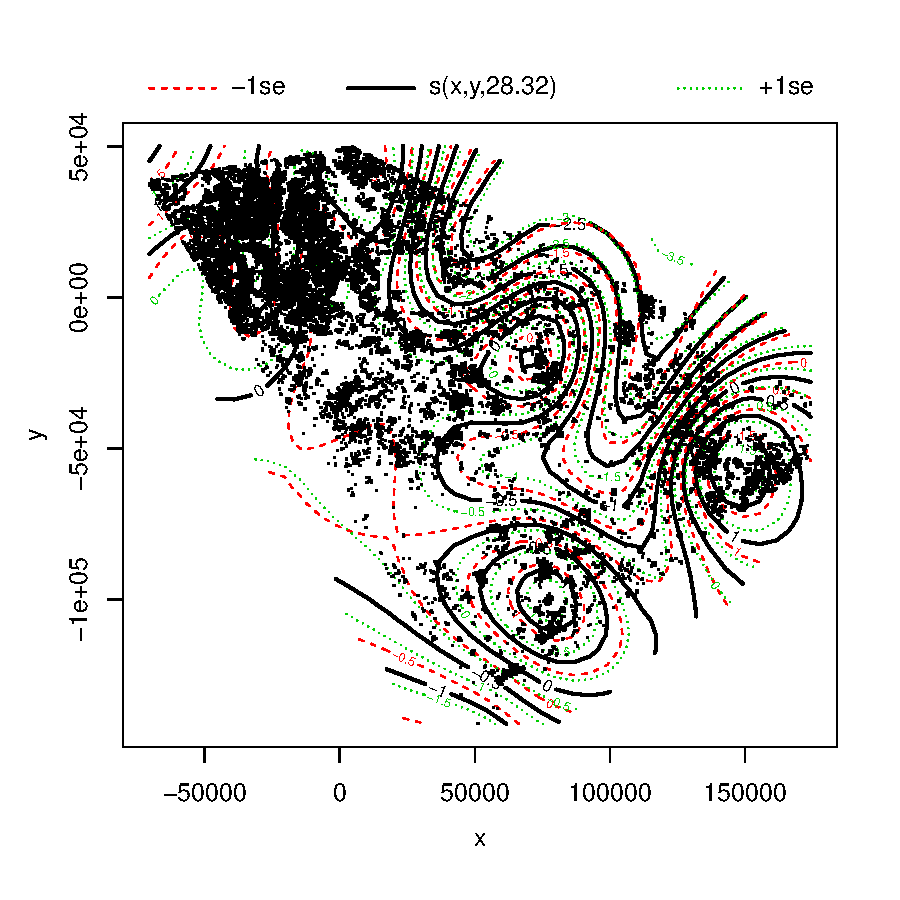
\includegraphics{HW9-002}
\end{figure}
Clearly there are 4 regions indicating high values of the predicted log(odds) given that other predictors (except the spatial coordinates $x$ and $y$) are held at zero. Since $log(odds_i)\propto p_i$, these regions have elevated risk of mistletoe presence.\\
This can be more easily interpreted with the following 3D plot showing 4 peaks and the colour plot (scheme 2) showing 4 lighter regions corresponding to high values.
\begin{figure}[H]
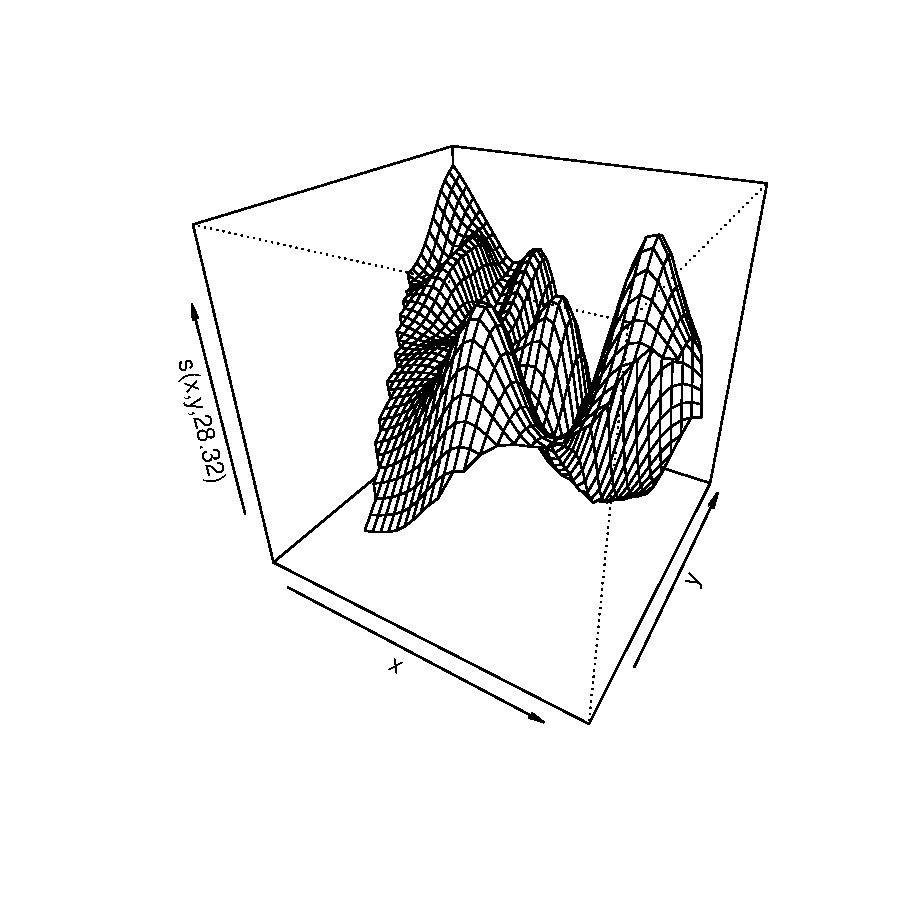
\includegraphics{HW9-003}
\end{figure}
\begin{figure}[H]
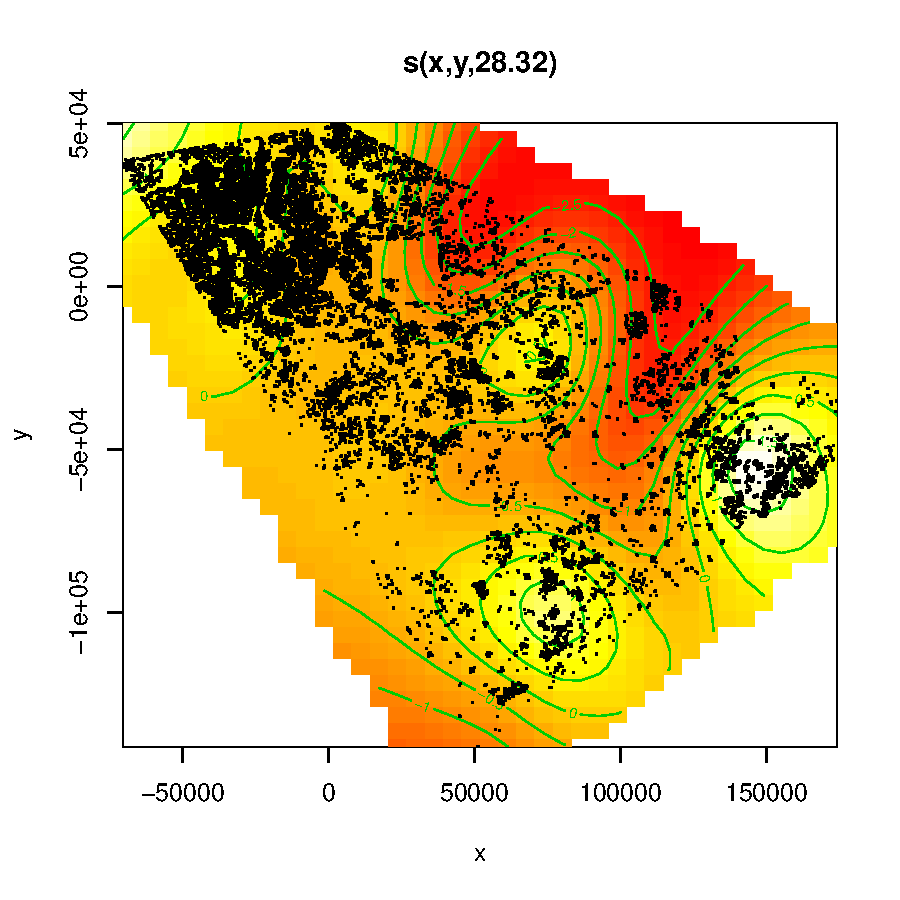
\includegraphics{HW9-004}
\end{figure}
This information might be very useful to the forest managers because if they know what forest stands are more prone to mistletoe presence they can take preventive measures to reduce the growth of mistletoe in these areas. Mistletoe is a parasitic plant and kills trees and so these preventive measures might help in conservation of natural habitats.
\en
\section*{Answer 2}
\bn
\item 
\begin{itemize}
\item Fitting Model 1: $\text{admit}_i \sim Bern(p_i)$, with $l(E(Y_i))=\eta_i+f(gre_i)+g(gpa_i)=X_i\beta+f(gre_i)+g(gpa_i)$ (l being the canonical logit link in bernoulli model)\\
$log(\dfrac{p_i}{1-p_i})=\beta_0+\beta_1 rank_i+f(gre_i)+g(gpa_i)$\\
\begin{Schunk}
\begin{Sinput}
> library(mgcv)
> admissions <- read.csv("http://www.ats.ucla.edu/stat/data/binary.csv")
> fit1=gam(admit~rank+s(gre)+s(gpa),data=admissions,family=binomial)
> summary(fit1)
\end{Sinput}
\begin{Soutput}
Family: binomial 
Link function: logit 

Formula:
admit ~ rank + s(gre) + s(gpa)

Parametric coefficients:
            Estimate Std. Error z value Pr(>|z|)    
(Intercept)   0.5386     0.3164   1.702   0.0887 .  
rank         -0.5631     0.1276  -4.413 1.02e-05 ***
---
Signif. codes:  0 ‘***’ 0.001 ‘**’ 0.01 ‘*’ 0.05 ‘.’ 0.1 ‘ ’ 1 

Approximate significance of smooth terms:
        edf Ref.df Chi.sq p-value  
s(gre) 1.00  1.000  4.318  0.0377 *
s(gpa) 2.97  3.713  8.273  0.0686 .
---
Signif. codes:  0 ‘***’ 0.001 ‘**’ 0.01 ‘*’ 0.05 ‘.’ 0.1 ‘ ’ 1 

R-sq.(adj) =  0.096   Deviance explained = 8.82%
UBRE = 0.16949  Scale est. = 1         n = 400
\end{Soutput}
\end{Schunk}
\item Fitting Model 2: $\text{admit}_i \sim Bern(p_i)$, with $l(E(Y_i))=\eta_i+g(gpa_i)=X_i\beta+g(gpa_i)$ (l being the canonical logit link in bernoulli model)\\
$log(\dfrac{p_i}{1-p_i})=\beta_0+\beta_1 rank_i+\beta_2 gre_i+g(gpa_i)$\\
\begin{Schunk}
\begin{Sinput}
> library(mgcv)
> admissions <- read.csv("http://www.ats.ucla.edu/stat/data/binary.csv")
> fit2=gam(admit~rank+gre+s(gpa),data=admissions,family=binomial)
> summary(fit2)
\end{Sinput}
\begin{Soutput}
Family: binomial 
Link function: logit 

Formula:
admit ~ rank + gre + s(gpa)

Parametric coefficients:
             Estimate Std. Error z value Pr(>|z|)    
(Intercept) -0.800502   0.743319  -1.077   0.2815    
rank        -0.563112   0.127610  -4.413 1.02e-05 ***
gre          0.002279   0.001097   2.078   0.0377 *  
---
Signif. codes:  0 ‘***’ 0.001 ‘**’ 0.01 ‘*’ 0.05 ‘.’ 0.1 ‘ ’ 1 

Approximate significance of smooth terms:
         edf Ref.df Chi.sq p-value  
s(gpa) 2.971  3.714  8.275  0.0686 .
---
Signif. codes:  0 ‘***’ 0.001 ‘**’ 0.01 ‘*’ 0.05 ‘.’ 0.1 ‘ ’ 1 

R-sq.(adj) =  0.096   Deviance explained = 8.83%
UBRE = 0.16949  Scale est. = 1         n = 400
\end{Soutput}
\end{Schunk}
\item AIC values of the above models can be computed as:
\begin{Schunk}
\begin{Sinput}
> AIC(fit1)
\end{Sinput}
\begin{Soutput}
[1] 467.7949
\end{Soutput}
\begin{Sinput}
> AIC(fit2)
\end{Sinput}
\begin{Soutput}
[1] 467.7948
\end{Soutput}
\end{Schunk}
Clearly the difference is of the order of $10^{-4}<<2$ which is insignificant and does not help in making any model selection decision. Plotting the smooth function $f(gre)$ in Model 1 as follows, we can notice that it looks very much linear.
\begin{figure}[H]
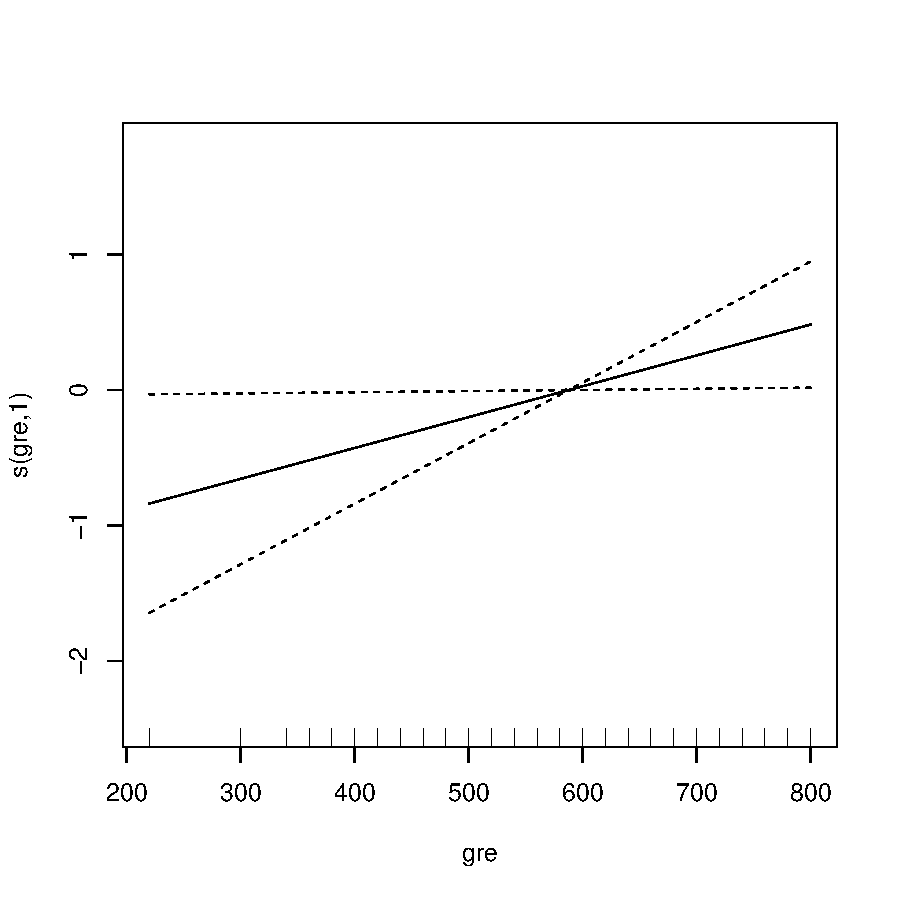
\includegraphics{HW9-008}
\end{figure}
This linear dependence of the f(gre) with respect to gre nullifies the effect of smoothing. Due to the absence of any non-linear dependence of f(gre) on gre, the two models are equivalent and this also accounts for the little difference in AIC values. 
\item Now the $log(odds)$ depends on gre linearly in Model 1 as can be seen from the previous graph. Thus the mean of admiitance is directly proportional to the gre score. Model 2 gives the same result. Futher the smooth function of gpa can be plotted as:
\begin{figure}[H]
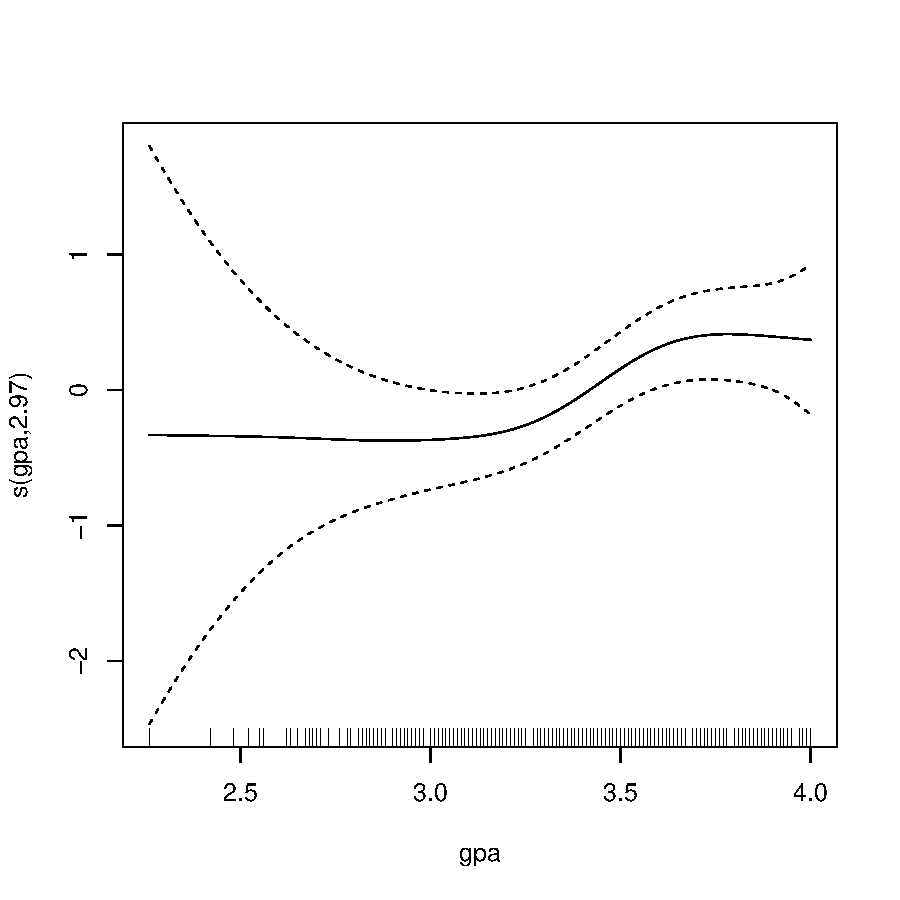
\includegraphics{HW9-009}
\end{figure}
This clearly shows that the log(odds) of admittance is constant below 3.3 gpa, varies approximately linearly with gpa for $3.3 \leq gpa\leq 3.6$ and again becomes roughly constant for $gpa \geq 3.6$. This implies that there is greater probability of admittance for $gpa \geq 3.5$ than for $gpa \leq 3.5$. Again this holds for both the models.
\end{itemize}
\en
\end{document}
